\section*{Диаграммы состояний и события}
\addcontentsline{toc}{section}{Диаграммы состояний и события}
\subsection*{Светофор}
\addcontentsline{toc}{subsection}{Светофор}

\textbf{Задание:}\\
Реализовать модели работы светофоров при помощи диаграммы состояний.\\

\textbf{Решение:}\\
Необходимо промоделировать работу двух светофоров -- дорожного и пешеходного. Сначала стоит нарисовать данные объекты. (Рисунок \ref{fig:traffic_light1})
\begin{figure}[h]
	\centering 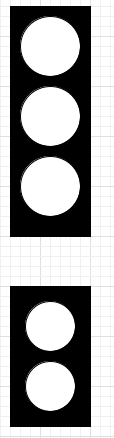
\includegraphics[scale=0.5]{traffic_light1}
	\caption{Визуальное отображение светофоров}
	\label{fig:traffic_light1}
\end{figure}

Далее была создана диаграмма действий, в которой реализована основная логика светофора. (Рисунок \ref{fig:traffic_light2})
\begin{figure}[h]
	\centering 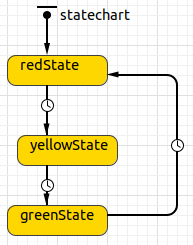
\includegraphics[scale=0.5]{traffic_light2}
	\caption{Диаграмма состояний светофоров}
	\label{fig:traffic_light2}
\end{figure}

Можно сказать что данная логика реализована относительно дорожного светофора.

\newpage

Все переходы модели осуществляются по таймауту. Рассмотрим логику работы светофоров, когда на дорожном светофоре горит красный свет. Мы назначаем дорожному светофору красный свет, а пешеходному назначаем зелёный. (Рисунок \ref{fig:traffic_light3})
\begin{figure}[h]
	\centering 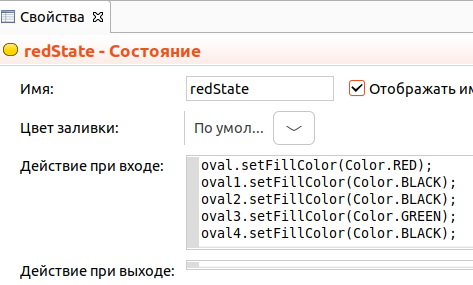
\includegraphics[scale=0.5]{traffic_light3}
	\caption{Пример логики одного из состояний}
	\label{fig:traffic_light3}
\end{figure}

Аналогично было проделано для жёлтого и зелёного состояний.\\

Таким образом, при помощи диаграммы состояний была промоделирована работа изменение сигналов дорожного и пешеходного светофоров.